\documentclass[a4 paper]{article}
% Set target color model to RGB
\usepackage[inner=2.0cm,outer=2.0cm,top=2.5cm,bottom=2.5cm]{geometry}
\usepackage{setspace}
\usepackage[rgb]{xcolor}
\usepackage{verbatim}
\usepackage{subcaption}
\usepackage{amsgen,amsmath,amstext,amsbsy,amsopn,tikz,amssymb,tkz-linknodes}
\usepackage{fancyhdr}
\usepackage[colorlinks=true, urlcolor=blue,  linkcolor=blue, citecolor=blue]{hyperref}
\usepackage[colorinlistoftodos]{todonotes}
\usepackage{rotating}
\usepackage{float}

\usepackage{booktabs}
\newcommand{\ra}[1]{\renewcommand{\arraystretch}{#1}}

\newtheorem{thm}{Theorem}[section]
\newtheorem{prop}[thm]{Proposition}
\newtheorem{lem}[thm]{Lemma}
\newtheorem{cor}[thm]{Corollary}
\newtheorem{defn}[thm]{Definition}
\newtheorem{rem}[thm]{Remark}
\numberwithin{equation}{section}

\newcommand{\homework}[6]{
   \pagestyle{myheadings}
   \thispagestyle{plain}
   \newpage
   \setcounter{page}{1}
   \noindent
   \begin{center}
   \framebox{
      \vbox{\vspace{2mm}
    \hbox to 6.28in { {\bf COL774:~Machine Learning \hfill { #2}} }
       \vspace{6mm}
       \hbox to 6.28in { {\LARGE \hfill #1  \hfill} }
       \vspace{6mm}
       \hbox to 6.28in {\bf {Entry Number: {\rm #4} \hfill Name: {\rm #5} } }
       % \hbox to 6.28in { {\it TA: #4  \hfill #6}}
      \vspace{2mm}}
   }
   \end{center}
   \markboth{#1}{#1}
   \vspace*{4mm}
}

% \newcommand{\problem}[2]{~\\\fbox{\textbf{Problem #1}}\hfill (#2 points)\newline\newline}
% \newcommand{\subproblem}[1]{~\newline\textbf{(#1)}}
% \newcommand{\D}{\mathcal{D}}
% \newcommand{\Hy}{\mathcal{H}}
% \newcommand{\VS}{\textrm{VS}}
% \newcommand{\solution}{~\newline\textbf{\textit{(Solution)}} }

% \newcommand{\bbF}{\mathbb{F}}
% \newcommand{\bbX}{\mathbb{X}}
% \newcommand{\bI}{\mathbf{I}}
% \newcommand{\bX}{\mathbf{X}}
% \newcommand{\bY}{\mathbf{Y}}
% \newcommand{\bepsilon}{\boldsymbol{\epsilon}}
% \newcommand{\balpha}{\boldsymbol{\alpha}}
% \newcommand{\bbeta}{\boldsymbol{\beta}}
% \newcommand{\0}{\mathbf{0}}

\begin{document}
\homework{Assignment 4 Report}{Date: April 26, 2019}{}{\bf 2016CS10363}{\bf Manish Tanwar}{NetId(s)}

\section*{Data Generation (For every part)}
The datapoints(image sequences) are generated with following procedure:
\begin{itemize}
    \item Chose every positive example with probability $4/5$.
    \item Negative examples are chosen with probability $1/20$.
    \item Each of the $6 \choose 2$ are chosen with probability $2/3$.
    \item Using these probablities the sequences generated are in following ratio:
    Positive vs. Neagative = $2:5$
\end{itemize}

\section*{Part 1: Fixed Algorithms:}
\subsection*{(A) PCA + SVM:}

\begin{enumerate}
    \item Libraries Used:
    \begin{itemize}
        \item Scikit-learn's PCA and Incremental PCA.
        \item Scikit-learn's SVM (SVC)
    \end{itemize}
    \item Preprocessing:
    \begin{itemize}
        \item Converted images to greyscale.
        \item Pixels values are normalised to $[0,1]$ by dividing by 255.
        \item Used Incremental PCA to transform down dimension to 50.
        \item For Incremental PCA : Batch Size = 100
        \item Variance Achieved = 82\%
    \end{itemize}
    
    \item Implementation Details:
    \begin{itemize}
        \item Stacked five frames of size (50) to get (250) as each data-point input.
    \end{itemize}

    \item \textbf{Linear Kernel:}
    \begin{itemize}
        \item Trained Linear Kernel on 30000 examples for 25000 iterations.
        \item On Validation data : F-score = 0.29
    \end{itemize}

    \item \textbf{Gaussian Kernel:}
    \begin{itemize}
        \item Trained Linear Kernel on 30000 examples for 25000 iterations.
        \item On Validation data : F-score = 0.08
    \end{itemize}

\end{enumerate}

\subsection*{(B) Convolutional Neural Network (CNN):}

\begin{enumerate}
    \item Libraries Used: \textbf{keras}
    \item Preprocessing:
    \begin{itemize}
        \item Pixels values are normalised to $[0,1]$ by dividing by 255.
        \item Cropped the image from (210,160,3) to (183,154,3) in the following manner:
        \begin{figure}[H]
            \centering
            % \hsapce*{1cm}
            \begin{minipage}[b]{0.4\textwidth}
              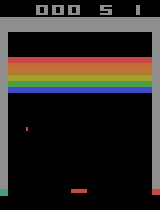
\includegraphics[width=0.6\textwidth]{extra/1.png}
              \caption{Original Image}
            \end{minipage}
            \hfill
            \begin{minipage}[b]{0.36\textwidth}
              
\includegraphics[width=0.7\textwidth]{extra/2.png}
              \caption{Cropped Image}
            \end{minipage}
          \end{figure}          
    \end{itemize}

    \item Architecture Details:
    \begin{itemize}
        \item Stacked five frames of size (183,154,3) to get (183,154,15) as each data-point input.
        \item Architecture specified in the problem statement is used.
        \item Optimizer = 'Adam'
        \item Learning Rate = 0.001
        \item Batch Size = 512
        \item Class Weights = \{1,7/4\} to get equal positive and negative examples.
    \end{itemize}

    \item \textbf{Results on Best Model:}
    \begin{itemize}
        \item Half of the provided Validation data used as test data and other half as validation data.
        \item Validation Data:
            \begin{itemize}
                \item F1-score = 0.49
                \item Accuracy = 95.67\%
            \end{itemize}
        \item Testing Data:
            \begin{itemize}
                \item F1-score = 0.56
                \item Accuracy = 96.34\%
            \end{itemize}
    \end{itemize}

\end{enumerate}

\section*{Part 2: Competition Part:}

\begin{enumerate}
\item Libraries Used: \textbf{keras}
    \item Preprocessing:
    \begin{itemize}
        \item Converted images to greyscale.
        \item Pixels values are normalised to $[0,1]$ by dividing by 255.
        \item Cropped the image from size (210,160,3) to (162,154,1) in the following manner:
        \begin{figure}[H]
            \centering
            % \hsapce*{1cm}
            \begin{minipage}[b]{0.4\textwidth}
              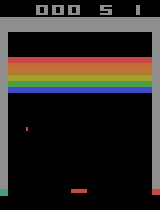
\includegraphics[width=0.6\textwidth]{extra/1.png}
              \caption{Original Image}
            \end{minipage}
            \hfill
            \begin{minipage}[b]{0.35\textwidth}
              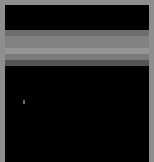
\includegraphics[width=0.7\textwidth]{extra/3.png}
              \caption{Cropped Image}
            \end{minipage}
          \end{figure}          
    \end{itemize}

    \item Architecture Details:
    \begin{itemize}
        \item Stacked five frames of (162,154,1) to get (162,154,5) as each data-point input.
        \item Architecture specified in the problem statement is used with Dropout(0.35) after the Dense layer.
        \item Optimizer = 'Adam'
        \item Learning Rate = 0.001
        \item Batch Size = 512
        \item Class Weights = \{1,7/4\} to get equal positive and negative examples.
        \item I trained three different models and predicted the value predicted by the majority of the models.
    \end{itemize}

    \item \textbf{Results on Best Model:}
    \begin{itemize}
        % acc: 0.9992 - f1: 0.9985
        \item Training Data:
            \begin{itemize}
                \item F-score = 0.9985
                \item Accuracy = 99.92\%
            \end{itemize}
        \item Validation Data:
            \begin{itemize}
                \item F-score = 0.5726
                \item Accuracy = 97.09\%
            \end{itemize}
        \item Testing Data(on kaggle):
            \begin{itemize}
                \item F-score = \textbf{0.5945}
            \end{itemize}
    \end{itemize}

\end{enumerate}
\end{document}